\documentclass{article}
\usepackage{graphicx} % Required for inserting images
\usepackage{enumitem}
\usepackage{amsmath}
\usepackage{amsfonts}
\usepackage{amssymb}
\usepackage{amstext}
\usepackage{mdframed}
\usepackage{hyperref}
\usepackage{multicol}
\usepackage{comment}
\usepackage{float}
\usepackage{listings}
\usepackage{subcaption}
\hypersetup{
    colorlinks=true,
    linkcolor=darkblue,
    filecolor=magenta,      
    urlcolor=blue,
    citecolor=violet,
    pdftitle={Overleaf Example},
    pdfpagemode=FullScreen,
}
\lstset{
  basicstyle=\ttfamily,
  columns=fullflexible,
}
\usepackage{bbm}
\usepackage[top = 1.5cm, left = 2cm, right = 2cm, bottom = 2cm]{geometry}
\setlength{\parindent}{0 in}
\setlength{\parskip}{0.1 in}

% \graphicspath{ {./Images/} }

\title{Advanced Machine Unearning: Programming Assignment 4}
\author{Tejas Sharma, Muskaan Jain, Ojas Maheshwari}
\date{Spring 2025}

\begin{document}
\maketitle
\section{Task 0: Environment Setup and Result Reproduction}
\begin{lstlisting}
Using device: mps

--- Model Architecture ---
EnergyRegressor(
    (net): Sequential(
    (0): Linear(in_features=784, out_features=4096, bias=True)
    (1): ReLU(inplace=True)
    (2): Linear(in_features=4096, out_features=2048, bias=True)
    (3): ReLU(inplace=True)
    (4): Linear(in_features=2048, out_features=1024, bias=True)
    (5): ReLU(inplace=True)
    (6): Linear(in_features=1024, out_features=512, bias=True)
    (7): ReLU(inplace=True)
    (8): Linear(in_features=512, out_features=256, bias=True)
    (9): ReLU(inplace=True)
    (10): Linear(in_features=256, out_features=128, bias=True)
    (11): ReLU(inplace=True)
    (12): Linear(in_features=128, out_features=64, bias=True)
    (13): ReLU(inplace=True)
    (14): Linear(in_features=64, out_features=32, bias=True)
    (15): ReLU(inplace=True)
    (16): Linear(in_features=32, out_features=16, bias=True)
    (17): ReLU(inplace=True)
    (18): Linear(in_features=16, out_features=8, bias=True)
    (19): ReLU(inplace=True)
    (20): Linear(in_features=8, out_features=4, bias=True)
    (21): ReLU(inplace=True)
    (22): Linear(in_features=4, out_features=2, bias=True)
    (23): ReLU(inplace=True)
    (24): Linear(in_features=2, out_features=1, bias=True)
    )
)
------------------------

Loading dataset from ./A4_test_data.pt...
Dataset loaded in 0.18s. Shape: x=torch.Size([100000, 784]), energy=torch.Size([100000, 1])
Using device: mps
Using device: mps

--- Test Results ---
Loss: 288.1554
--- Script Finished ---
\end{lstlisting}
We set \texttt{DATASET\_PATH=`./A4\_test\_data.pt'} and loaded the state dictionary of the \texttt{EnergyRegressor} model from \texttt{MODEL\_WEIGHTS\_PATH=`./trained\_model\_weights.pth'}. Above is the output on running \texttt{get\_results.py}.

The files \texttt{A4\_test\_data.pt} and \texttt{trained\_model\_weights.pth} are downloaded from the assignment drive link, and pasted onto the directory containing the python script \texttt{get\_results.py}.

\section{Task 1: MCMC Sampling Implementation}
We imported from the task 0 file \texttt{get\_results.py}, the \texttt{EnergyRegressor} class. We also used the \texttt{TSNE} class from \texttt{sklearn.manifold} to visualize the samples generated by the MCMC sampling algorithm that we implemented. Lastly, we imported the \texttt{clock\_gettime} function from the \texttt{time} library to measure the time taken by our sampling algorithms. The file for task 1 is \texttt{sampling\_algos.py}.

We assume that this file is in the same directory as the task 0 file, and also has the trained model weights file. On executing this file, we got the following output:
\begin{lstlisting}
Using device: mps
--- Sampling Times ---
Algo-1 Burn-in Time: 26.6275 seconds
Algo-1 Completion Time: 48.6032 seconds
Algo-2 Burn-in Time: 10.4676 seconds
Algo-2 Completion Time: 21.3794 seconds
\end{lstlisting}

We found that the best results were obtained on setting the value of burn-in to 1000 (1000 samples pre-generated before actual sampling), and 1000 samples were generated after that, which were plotted. The value of $\tau$ or the learning rate is set to 0.01.

Above results were generated using these hyperparameters. It is evident that the second algorithm is more than twice as fast as the first, which is understandable considering that we do not evaluate any function (probabilistic) that decides whether we reject or accept the new sample.

\subsection{2D and 3D visualization of generated samples}
\begin{figure}[H]
    \centering
    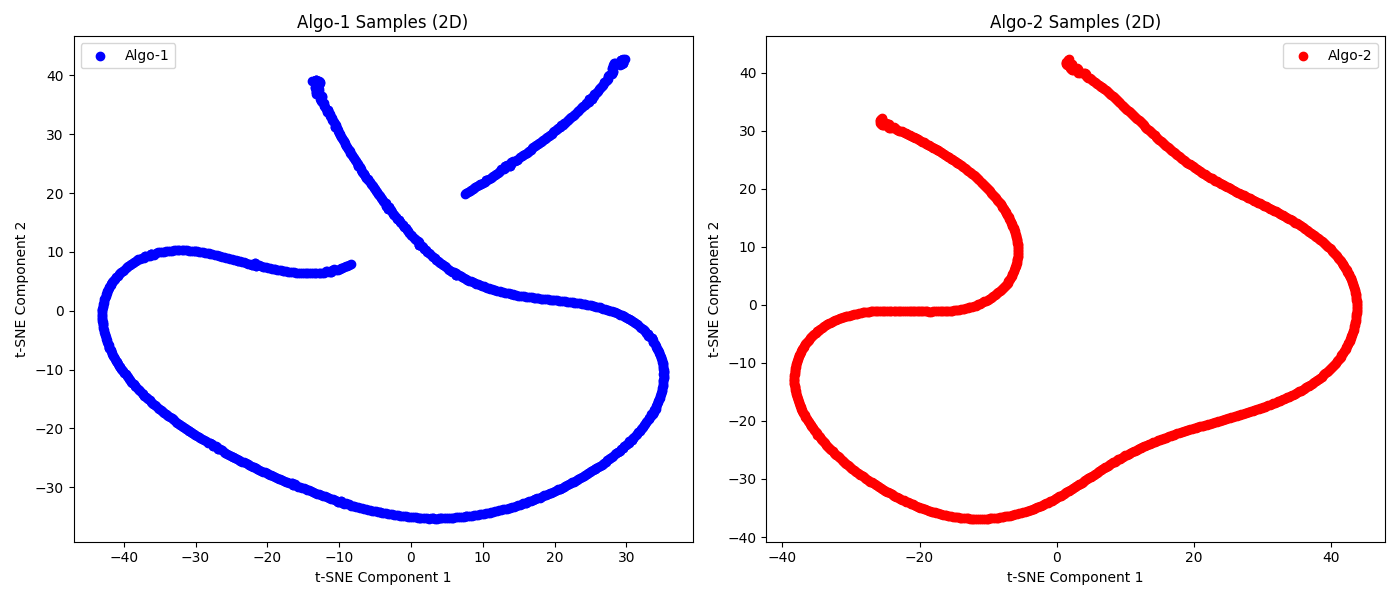
\includegraphics[width=\linewidth]{TASK-0-1/algo_samples_2d.png}
    \caption{2D visualization of generated samples}
    \label{fig:2d_samples}
\end{figure}
\begin{figure}[H]
    \centering
    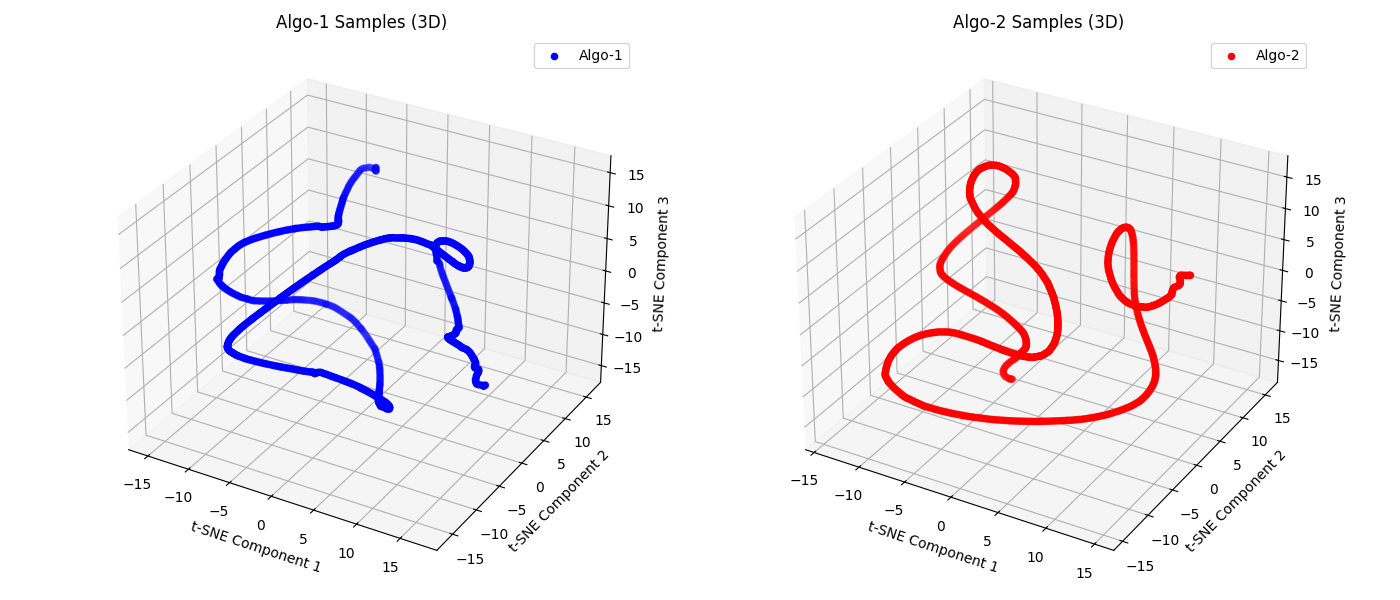
\includegraphics[width=\linewidth]{TASK-0-1/algo_samples_3d.png}
    \caption{3D visualization of generated samples}
    \label{fig:3d_samples}
\end{figure}

\end{document}